%\chapter{Rationale of Designing RDF engine for Edge nodes}






\chapter{Flash-Aware RDF Storage}
\label{ch:rdfstorage}
\lhead{Chapter~\ref{ch:rdfstorage}. Flash-Aware RDF Storage}


This section provides the design of physical organisation of RDF storage for IoT edge devices.

%---------------------------------------------------------------------------------%
\section{Architecture Overview}
\label{s:ao}
\lhead{\ref{s:ao}. Architecture Overview}


\begin{figure}[ht!]
   \centering
   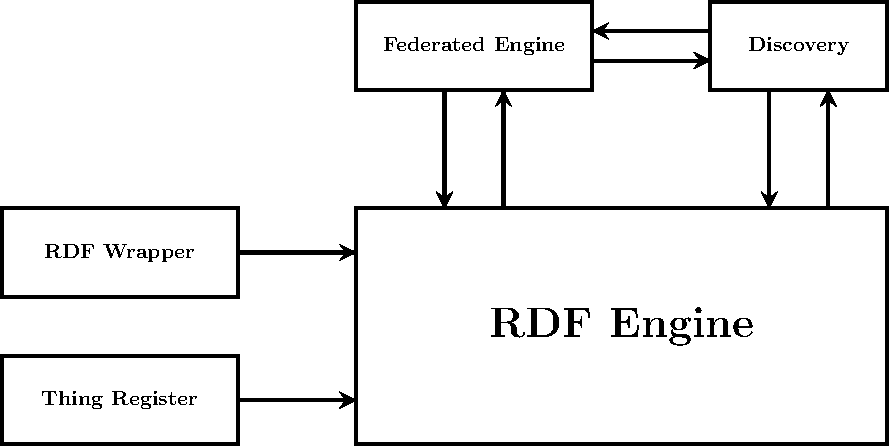
\includegraphics[width= 0.35\textwidth]{c5/arch}
     \caption{System Architecture Overview}
   \label{fig:arc_ove} 
\end{figure}




\section{RDF Physical Storage Design}
\label{sec:c4-retionale}

The physical organisation heavily influences the write performance, read performance and space utilisation of a database~\citep{Ullman:2001}. 
The selection of physical organisation for a database is also impacted by the type of storage medium that the database targets~\citep{Owens:2011}.
From the findings in Chapter~\ref{}, the schemes for storing RDF data on a workstation -- as described in Section~\ref{} -- cannot be deployed on the IoT edge devices.
Therefore, it is required to design an alternative physical organisation for RDF data that is well-suited the characteristic of hardware characteristic of IoT edge devices (presented in Section~\ref{}) and also provides high insert throughput for the RDF engines.

As we already mentioned in Section~\ref{}, RDF triples can be stored following the approach of multiple-indexing techniques~\citep{}.


%In order to store RDF data, we following the approach of creating access patterns for RDF triples as described in Section~\ref{sec:phy_sto}. For every RDF graph(dataset), three Triple lists, namely subject-predicate-object (SPO), predicate-object-subject (POS), object-subject-predicate (OSP), are created. 
%With this schema, for any combinations of subject, predicate, or object, a corresponding list, which is suitable for retrieving related triples, can be found in these three lists. Several RDF stores do implement all six of the possible indexing orderings over RDF data such as Hexastore~\cite{Weiss:2008} or YARS~\cite{Harth:2005}. However, using three combinations of nodes in a cyclic ordering is enough to cover all query patterns. This indexing schema is not efficient for answering complex queries~\cite{Weiss:2008}; however, to compare with other schemes, this costs lower resource for updating and consumes smaller storage space.


Following the approach of multiple-indexing, RDF4Led
stores RDF triples in three storage layouts as sorted permu-
tations of triples: SPO (Subject - Predicate - Object), POS,
and OSP. 
Three permutations are sufficient to cover all query patterns, e.g., the SPO layout can be used to cover the triple query patterns with the bound subject (s ? ?) and the bound
subject-predicate (s p ?). 
Although, storing all six combinations may answer complex queries more effectively, using only three consumes less storage space and decreases the cost of updates, i.e., we must update only three data structures instead of six, which is crucial for flash storage.

To reduce the memory required to maintain the index of data in flash storage, we use an alternative index structure that is based on the Block Range Index(BRIN) approach [20]. 
The basic idea of BRIN is to summarise the information of a data block of persistent storage (e.g. its location) into a small tuple. 
The result is that we minimise the amount of memory required to maintain the index of the data.


Specifically, we introduce a \emph{Physical Layer} and a \emph{Buffer Layer}. 
The Physical Layer stores data directly on flash storage (Physical RDF Storage) and the Buffer Layer operates in the main memory (Buffer Manager) and has the following main roles: 
\begin{itemize}
\item (i) grouping and caching atomic data updates before writing a block; 
\item (ii) indexing the data stored on the Physical Layer 
\item (iii) caching recently used data for read performance. This allows us to group multiple updates within a block into one erase-and-write operation and to improve read performance through the cache.
\end{itemize}

\begin{figure}[ht!]
	\centering
    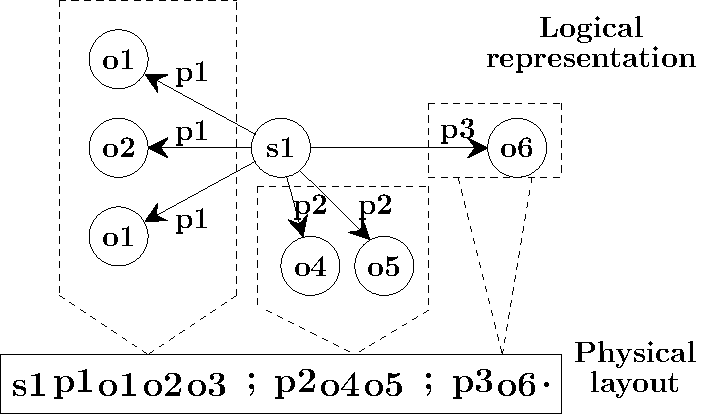
\includegraphics[width=0.5\textwidth]{c5/molecule.pdf}
    \caption{Logical and physical representation of a molecule.}
    \label{fig:molecule}
\end{figure}

\subsection{Physical Layer:}  

To achieve high compression of triples on the flash storage we leverage the molecule-based storage model. 
RDF molecule is a hybrid data structures, it stores a compact list of properties and objects related to a subject, i.e., the root of the molecule.
Molecule clusters are used in two ways: to logically group sets of relates resources, and to physically co-locate information related to a given object. 
Physically we represent a molecule as a list of co-located integers corresponding to S, P, and O (Figure~\ref{fig:molecule}). 
In such a way, we avoid storing repetitive values multiple times. Moreover, we enable further data compression, e.g., by storing deltas of sorted integers instead of full values.


In Physical Layer, we store sorted molecules into contiguous pages (read units) which are grouped into blocks (erase units). Moreover, all entities in molecules are also sorted to improve search performance. In this example depicted on Figure~\ref{fig:index}, each block in the Physical Layer contains four pages and each page stores molecules. 

\subsection{Buffer Layer:}

Similarly to the idea of BRIN, the Buffer Layer summaries the information of the data in the Physical Layer.
In the Buffer Layer, we keep the information about the first triple of a molecule in a page and the first page in a block. Figure~\ref{fig:index} depicts an example of the indexing structure that uses for storing an SPO index. The Buffer Layer maps physical addresses of pages and blocks, thus it acts as an index for the Physical Layer. We distinguish three types of an entry in the Buffer Layer: tuple entry, page entry and block entry. A \emph{page entry} is an entry that refers to the beginning of a page in the Physical Layer, it contains the first triple in the first molecule of the page. A \emph{block entry} is a page entry with an extra field indicating that this page is the first page a block. A \emph{tuple entry} contains an atomic triple and a value indicating whether this triple has been modified. In the Figure~\ref{fig:index}, the gray columns represent block entries and white columns represent page entries. For fast lookups on Buffer Layer, all triples are sorted.  Moreover, we maintain the logical order of the triples as in the Physical Layer. This allows us to group and commit sequential pages containing modified triples and belonging to the same block, within one write operation.

\begin{figure}[ht!]
\centering
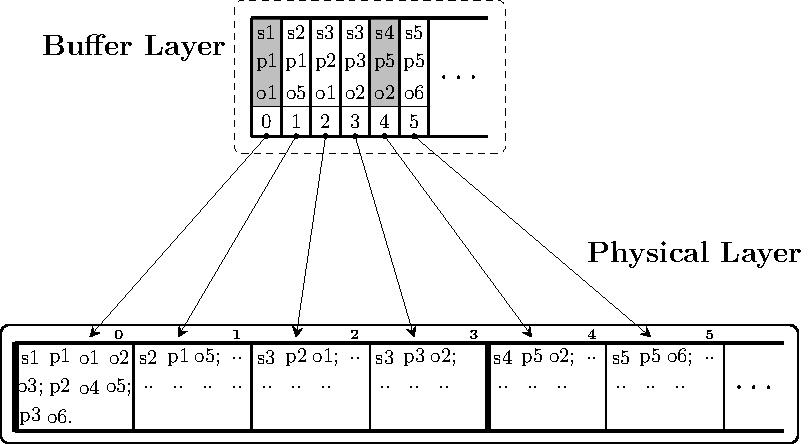
\includegraphics[width=.7\textwidth]{c5/index.pdf}
\caption{Two-layers storage model consist of a Physical Layer and a Buffer Layer.}
%The Physical Layer stores data on flash storage in a form of compact molecules.}
%The Buffer Layer manages changes in data,  caches changes in main memory, indexes data on Physical Layer, and caches data for reads. The Buffer Layer manages changes in data,  caches changes in main memory, indexes data on Physical Layer, and caches data for reads.
\label{fig:index}
\end{figure}

%---------------------------------------------------------------------------------%
\section{Index lookup} 

To retrieve RDF triples that match a triple pattern we execute a lookup on a corresponding layout of molecules. For example, a triple pattern (s, p, ?) is executed on the SPO layout or a triple pattern (?, p, o) is executed on the POS layout. As triples are sorted, the matched tuples are retrieved as a sublist. For instance, the matched tuples of the triple pattern (s, p, ?) are the tuples on the SPO layout which are of a form (s, p, o$_{i}$) and they are located between (s, p, o$_{min}$) and (s, p, o$_{max}$), where o$_{min}$ and o$_{max}$ are the smallest and the greatest object's identifiers within the layout. In other words, the sublist is computed by finding the lower and the upper bound positions of the matched tuples on the layout.
As in the example, the lower bound position of the matched sublist is the position of the tuple (s, p, o$_{min}$) and the upper bound position is the position of the tuple (s, p, o$_{max}$).
The matched triples are extracted from the layout by probing the range tuple by tuple from the lower to the upper bound positions. 

A position of a tuple is identified with a page, a molecule, and the exact position of the tuple within the page. To search for the lower bound position, we replace variables of the triple pattern with Integer$_{min}$ (the minimal integer value that can be used as an ID) and we do a simple search with the tuple. For the upper bound, we replace the variables by Integer$_{max}$ (the maximal integer value that can be used as an ID).
The search first finds the page that contains the tuple by searching in the Buffer Layer. 
The page entries within the Buffer Layer points to the first triple of the first molecule of each page, such entries are also sorted. Therefore, to find a page we perform a binary search over the page entries in the Buffer Layer. Then, we read the page from the Physical Layer and we perform the second binary search to find the exact position of the tuple within the page. 

For instance, to lookup of triple query pattern (09, ?, ?) is executed on the SPO layout depicted on Figure~\ref{fig:index}. The first tuple of the sublist is the first tuple that is greater than or equal to the triple (09, Integer$_{min}$, Integer$_{min}$) and the last tuple of the list is the first tuple that is smaller than or equal to the triple (09, Integer$_{max}$, Integer$_{max}$). 

With binary search over the Buffer Layer, we determine the physical pages containing the boundaries of the sublist:

\begin{itemize}
\item the lower bound within page 2 since (08, 07, 09) on the is the first tuple smaller than (09, Integer$_{min}$, Integer$_{min}$), and the page 3 starts already a tuple that is greater than (09, Integer$_{min}$, Integer$_{min}$) , i.e., (09, 05, 10);
\item the upper bound within page 8, since (09, 13, 01) is the first tuple smaller than  (09, Integer$_{max}$, Integer$_{max}$) and page 9 starts with a tuple greater than (09, Integer$_{max}$, Integer$_{max}$), i.e., (15, 6, 16). 
\end{itemize}

To find the exact positions of the lower and the upper boundaries we perform a second binary search withing pages 2 and 8. We find that the lower bound is on the second position within the  page 2. In case where tuple (09, Integer$_{min}$, Integer$_{min}$) was greater than the last tuple of page 2, the binary search would continue from the first tuple of page 3. Then, we find that the upper bound is on the first position within the  page 8. The last tuple of page 8 cannot be greater that (09, Integer$_{min}$, Integer$_{min}$) because in the Buffer Layer it is shown that the page 9 starts with (15, 06, 16). 
In consequence, we determine the physical boundaries of the sublist with tuples for our triple patterns (09, ?, ?) as: 

\begin{itemize}
\item the lower bound - the second position within the page 2
\item the upper bound - the first position within the page 8
\end{itemize}

In order to retrieve the results, we first load to the Buffer Layer the pages corresponding to the lower bound of the sublist, the triples from this page are then read one by one starting from the lower bound position. Then, we execute a similar process for all consecutive pages indicated by the page entities up to the page corresponding to the upper bound of the sublist. The process is halted at the position of the upper bound within the last page. The intermediate pages contribute to the results with all their triples. For our example, we load page 2 to the Buffer Layer, and we start retrieving triples from the second position of this page (the lower bound), then we load page 3 and we retrieve all its triples (intermediate page). Finally, we load page 8 and we retrieve only its first triple (the upper bound).

\section{Write Manager}

The write from Buffer Layer to Physical Layer is managed to adapt to the I/O behaviors of flash memory by the following basic principles: (i) minimise the number of physical writes to physical storage; (ii) group multiple updates within one write operation; (iii) keep a relatively high hit ratio for the data in the buffer. We use the Buffer Layer to delay write operations and to group many updates in blocks, hence, to mitigate the issue of single erase-before-write operations. For the high hit ratio, we keep the data block with the higher chance to be accessed and modified in the future. 

In order to keep track on the access frequency among blocks, we divide the buffer into two parts: cold and hot. In the hot part, we keep blocks that have been recently accessed, hence we do not want to move them to the Physical Layer. We organize data in a flat fashion within the hot part, i.e., we keep sorted triples instead of molecules to speed up atomic updates. The cold part contains molecule blocks that can be moved to the Physical Layer. When we access a block from the cold part or from the Physical Layer, we place it in the hot part of the Buffer Layer. 

The blocks are released from the hot part to the cold part and from the cold part by the following prioritised 
criteria: (i) the clean/unmodified blocks; (ii)the block with higher number of atomic triples in buffer; (iii) the higher density blocks, define by the ratio between the number of triples in a block and the capacity of the block i.e: $density_{Block A} = \frac{\#triples_{Block A}}{capacity_{Block A}}$; (iv) the last recently used blocks.   

\begin{figure}[ht!]
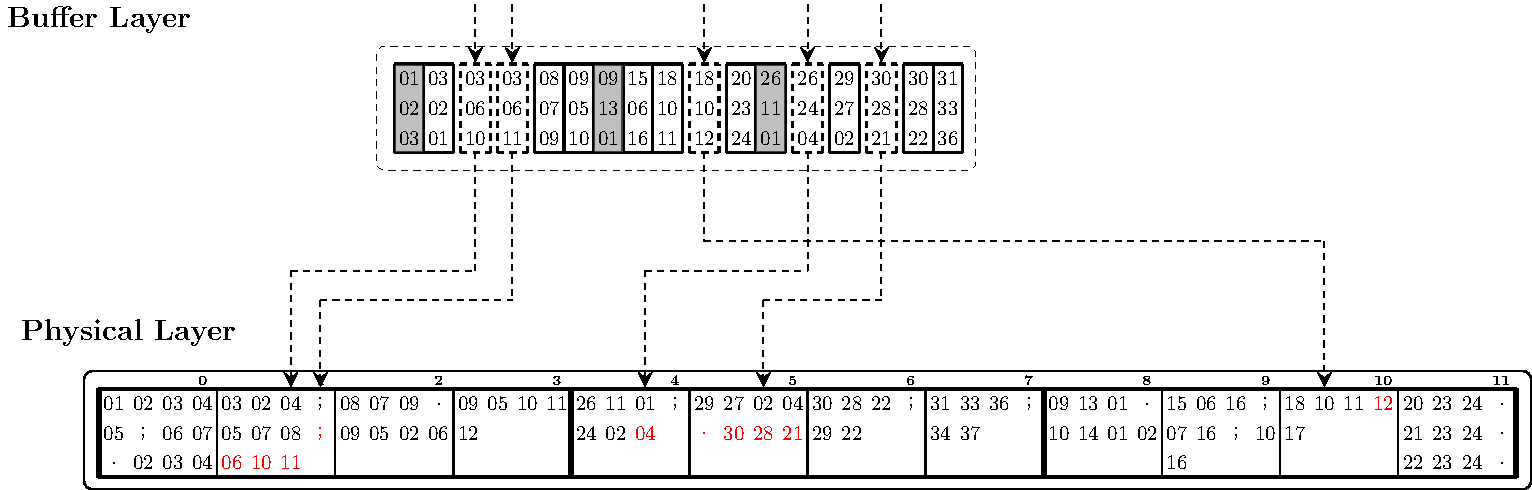
\includegraphics[width=1\textwidth]{c5/insert.pdf}
\caption{Example of inserting}
\label{fig:insert}
\end{figure}

Such order allows us to keep dirty/modified blocks in the buffer as long as possible in order to delay write operations and group more updates within dirty blocks. In case we need to release memory, we always refer to the cold part and we begin from the begin of the priority list. In consequence, we prioritize clean/unmodified blocks, as we do not have to perform any write operation for them, we just release the memory they occupy. Then, we prioritise blocks that contain many triples, i.e., high-density blocks, as they group multiple updates into one erase-write operation. 

For example, in Figure~\ref{fig:insert} illustrates the process of inserting 5 triples (03, 06, 01), (03, 06, 04), (18, 10, 12), (26, 24, 04), and (30, 28, 21). We first add them to the Buffer Layer; the page entries in the Buffer Layer indicate pages where the triples will be physically inserted. Triples (03, 06, 01), (03, 06, 04) are lexicographically smaller than the triple (08, 07, 09) which is the page entry mapping page 2 hence, they are added to page 1. Similarly, triple (18, 10, 12), (26, 24, 04) and (30, 28, 21) are will be added respectively to page 10, page 4, and page 5. 

When the size of the Buffer Layer reaches its limit or when data need to be moved to free memory, the triples are written to the Physical Layer. All dirty pages, i.e., pages containing modified tuples, within the same block are written at the same time to same expensive erase operations. For example, when the system needs to write 2 triples from buffer to storage, we move either data belonging to block 0, i.e., triples (03, 06, 01), (03, 06, 04), or data belonging to block 1, i.e., triples (26, 24, 04), (30, 28, 21), so that only one block is erased. In case we choose tuples (18, 10, 12) and (30, 28, 21), the system would have to erase two blocks before writing the data. Moving data from the Buffer Layer to the Physical Layer is essentially an optimization problem of maximizing the number of triples we can write within the minimal number of blocks in order to minimize the number of erase operations. Of course, block 0 is written before block 1 as its density is greater than that of block 1. The higher density means the less chance that the next triple will be dropped into that block.




\section{Evaluation Result}

\section{Summary}


%\section{Summary}


%As emphasized in the previous chapter, the design of existing mobile RDF triplestores exhibits several problems for the efficient storage and retrieval of RDF data on mobile devices. These designs are due to a lack of awareness of the small memory on mobile devices or distinctive I/O behaviour of flash storage. In order to overcome such issues, we consider creating a new design for mobile RDF triplestores.


%This chapter outlines our design for an efficient mobile RDF triplestore and improved techniques and strategy for storing RDF data. 
%Our design takes consideration from the ...
%he overview architecture of the mobile RDF triplestore and its building blocks are briefly described in Section~\ref{sec:c4_arch_overview}. In Section~\ref{sec:node_dic}, we discuss our strategy for reducing the memory consumption for representing RDF data in main memory by using an encoded dictionary. The selected physical organisation of mobile RDF storage is depicted in Section~\ref{sec:phy_org}.





























\nop{
Regarding the I/O cost of HERMES, suppose that available memory is M memory pages.
During the merging phase, M −1 memory pages are used for reading the input and 1
page is used to write to the output run. If the total size of the input tree is T memory
pages then each initial run will have an average size of 2(M − 1). Also, since
M − 1 buffers can be used for merging, there are going to be dlogM−1
d
T
2(M−1)
ee levels
of merging. Adding the first pass over the input to create the initial runs, we
have that there will be 1 + dlogM−1
d
T
2(M−1)
ee passes over the input. In each of these
passes, the whole tree is read and written to disk. This makes a total I/O cost of
2T ·

1+dlogM−1
d
T
2(M−1)
ee
.
As pointed out in [Graefe, 1993], one of the main concerns with replacement selection
is how one can handle the payloads of the nodes that reside in main memory
at any given time, i.e., the payloads of the nodes whose keys are in the heap at that
time. If these nodes are kept in the original buffer pages there is a great waste of space:
only half of the nodes of any given page are expected to be in the priority heap of their
parent node at any given point in time. This would mean that half of the available
memory is not effectively used for sorting keys. Therefore, the benefits from replacement
selection are cancelled (and quicksort could be used instead, probably yielding
better results). As also pointed out in [Graefe, 1993], the solution to this problem is
to copy the payloads of those nodes to a temporary space in memory until they are
written to the run, so that no space is wasted. Assuming that nodes of the same type
have similar size, this can be a viable solution. However, large variations in the size
of the nodes of the tree require complex and potentially overhead-inducing in-memory
management primitives.

Double buffering certain pages during the merging process is also a technique that
can improve the performance of our algorithm. For instance, using more than one
memory pages for the output run at each merge level can eliminate the need for the
CPU to wait for a write I/O call to complete after the output buffer is flushed (as is
the case if a single output buffer is used). Regarding the input buffers, the situation
is somewhat different. Reserving two memory pages (or more) per input run would
reduce the number of runs we can merge by half. What we can do is reserve a number
of k memory pages in order to prefetch the next page from the k input buffers that
contain one of the k smallest maximum keys among all buffers (since we then know
that the next page to be read will be the next from one of those k runs).

}



